\chapter{Benthic Habitat Mapping}
\lhead{Benthic Habitat Mapping}
\label{Benthic-Habitat-Mapping}
			
	\section{Gaussian Process Classifiers for Benthic Habitat Mapping}
	
	\section{Benthic Habitat Modeling}
	\label{ModelingOceanEnvironment:ModelingFeatures}
	
		This thesis project can be broken down into two main parts - ocean environment modeling and path planning. Ocean environment modeling itself includes bathymetric feature extraction and modeling, and environment label modeling. This section will focus on the environment modeling aspect.
			
		In order for autonomous underwater vehicles to plan a path that can maximise the amount of information gained regarding a particular ocean region, it would need a method to predict the types of environments it may encounter, with a measure of its prediction uncertainty.
		
		While the path planner is to plan in the spatial space, in general the prediction model operates upon some feature space with more direct and explicit relationships with the output we would like to predict.
		
		It is thus important to make a distinction between the feature space $F$ for which label modeling is to occur and the spatial space $S$ for which bathymetric modeling and planning is to occur. The spatial space usually consists of Cartesian coordinates $(x, y)$ in the eastings-northings frame or the longitude-latitude frame. The path is to be planned in this spatial space. The frame is usually converted into a local body frame during the execution of control signals for path tracking. However, this does not affect the formulation presented here. The feature space includes bathymetric features for which the labels will be modeled upon. Depending on the features employed for the modeling process, there are usually approximate analytical forms for extracting such features from raw depth observations.

		The following features in \cref{Background:OceanEnvironmentModeling:Table:Features} were chosen by the author for bathymetric modeling. 

		\begin{table}[h]
			\begin{center}
				\begin{tabular}{ |c|c|c| }
					\hline
					Feature Name & Feature Symbol & Feature Units \\
					\hline
					Depth & $h$ & m \\
					Slope (Small Scale) & $m_{s}$ & m/m \\
					Slope (Large Scale) & $m_{l}$& m/m \\
					Rugosity (Small Scale) & $r_{s}$ & $\mathrm{m^{2}/m^{2}}$ \\
					Rugosity (Large Scale) & $r_{l}$ & $\mathrm{m^{2}/m^{2}}$  \\
					\hline
				\end{tabular}
			\end{center}
	  	\caption{Bathymetric Features}
	  	\label{Background:OceanEnvironmentModeling:Table:Features}			
	  	\end{table}	
		
		The raw bathymetric data contains depth information at various spatial locations. Such data are often collected rather uniformly in approximate grid formations such that it is possible to calculate the ocean floor slope through finite differencing. The slope is divided into small scale and large scale variations, as marine environments - especially underwater habitats - often depend not only on the immediate slope but also slope variations on the larger scale. The same idea applies to rugosity, the measure of local height variations. The feature extraction process is detailed in \cref{Background:OceanEnvironmentModeling:FeatureExtraction}. 
		  
		Spatial coordinates are chosen to be excluded from the bathymetric feature set. For environment prediction purposes, it is expected that ecological habitats and geological sites exhibit no explicit relationship with the location of the site, and that its properties arise solely due to the local environment characteristics (features) of that site.
		
		\FloatBarrier			
		
		Figure \ref{Background:OceanEnvironmentModeling:Figure:modelingprocess} show a high level overview of the ocean environment modeling process. As bathymetric data is available in more quantities and distributed more uniformly, it is often sufficient to employ the feature extraction process outlined in \cref{Background:OceanEnvironmentModeling:FeatureExtraction} to obtain the bathymetric features for modeling. However, if the bathymetric data is sufficiently sparse or is not distributed uniformly for grid based methods, then the feature extraction process itself becomes a prediction problem.

		\begin{figure}[!htbp]
			\centering
				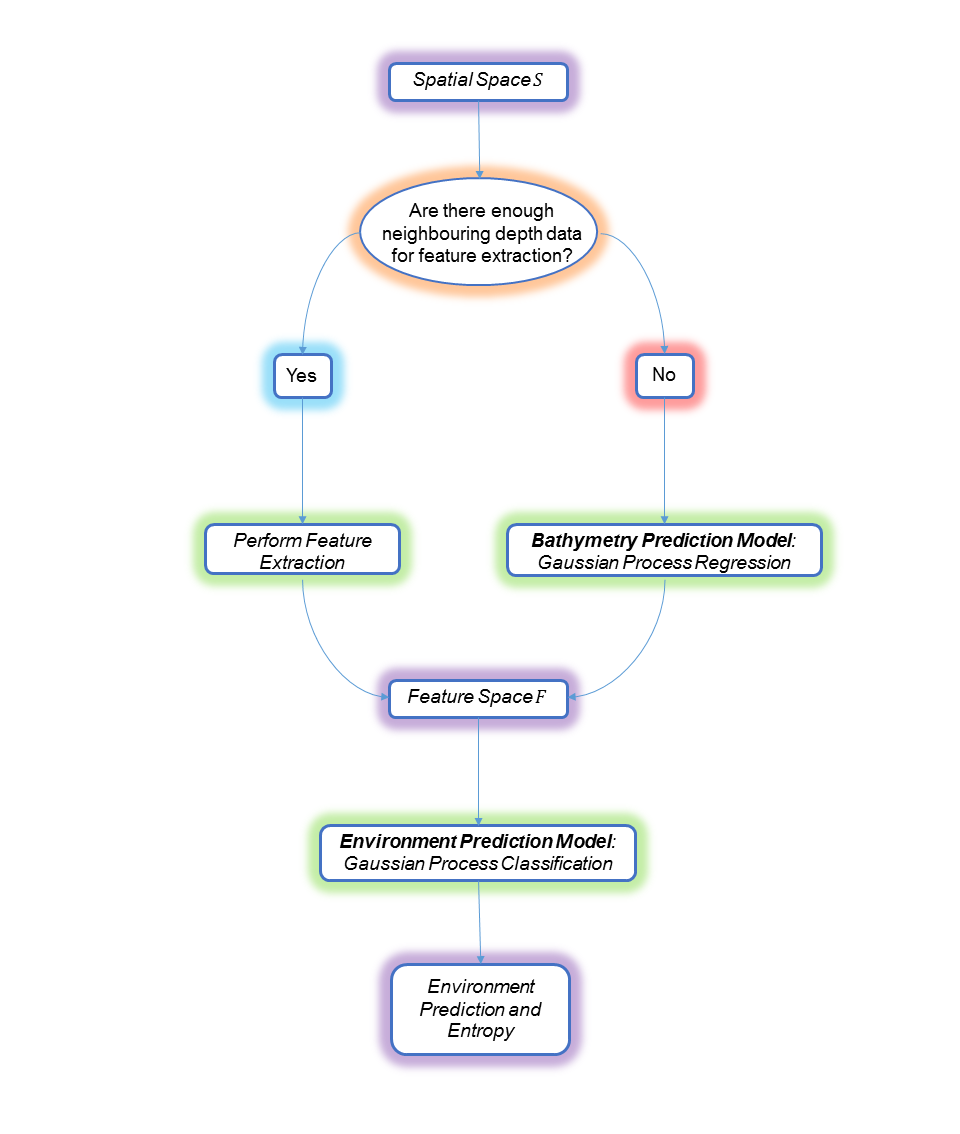
\includegraphics[width=\textwidth]{Figures/modelingprocess.png}
			\caption{Environment Modeling}
			\label{Background:OceanEnvironmentModeling:Figure:modelingprocess}
		\end{figure}
				
		In that case, a Gaussian process regression model is proposed for predicting the features at a given spatial location. While this is much more computationally expensive than performing feature extraction, it is also quite rare that this is necessary under abundant bathymetric data.
		
		Finally, once the feature vectors are obtained at training locations, the environment type is to be predicted. The environment type is summarised through labels that indicate the type of marine environment that was observed or predicted. Common AUV mission examples include "reef", "sand", and "rocks". These labels are often summarised through processing visual and stereo imagery obtained through past AUV missions. With a discrete set of possible labels, the environment prediction problem is to be modeled as a Gaussian process classification problem. From here on, the environment prediction problem is understood to refer to the two stage process of feature extraction or modeling and environment label prediction, with the latter being the main bottleneck for this process.
		
		\FloatBarrier
		
		\subsection{Data Matching}
		\label{Background:OceanEnvironmentModeling:DataMatching}
		
			A subtlety that arises from the above formulation is that during the training stage, the bathymetric data and the label data are not necessarily observed at the same places. Figure \ref{Background:OceanEnvironmentModeling:Figure:illustrationBathymetricAgainstLabels} illustrates the spatial distribution of the two datasets in a typical setting.
		
			\begin{figure}[!htbp]
				\centering
					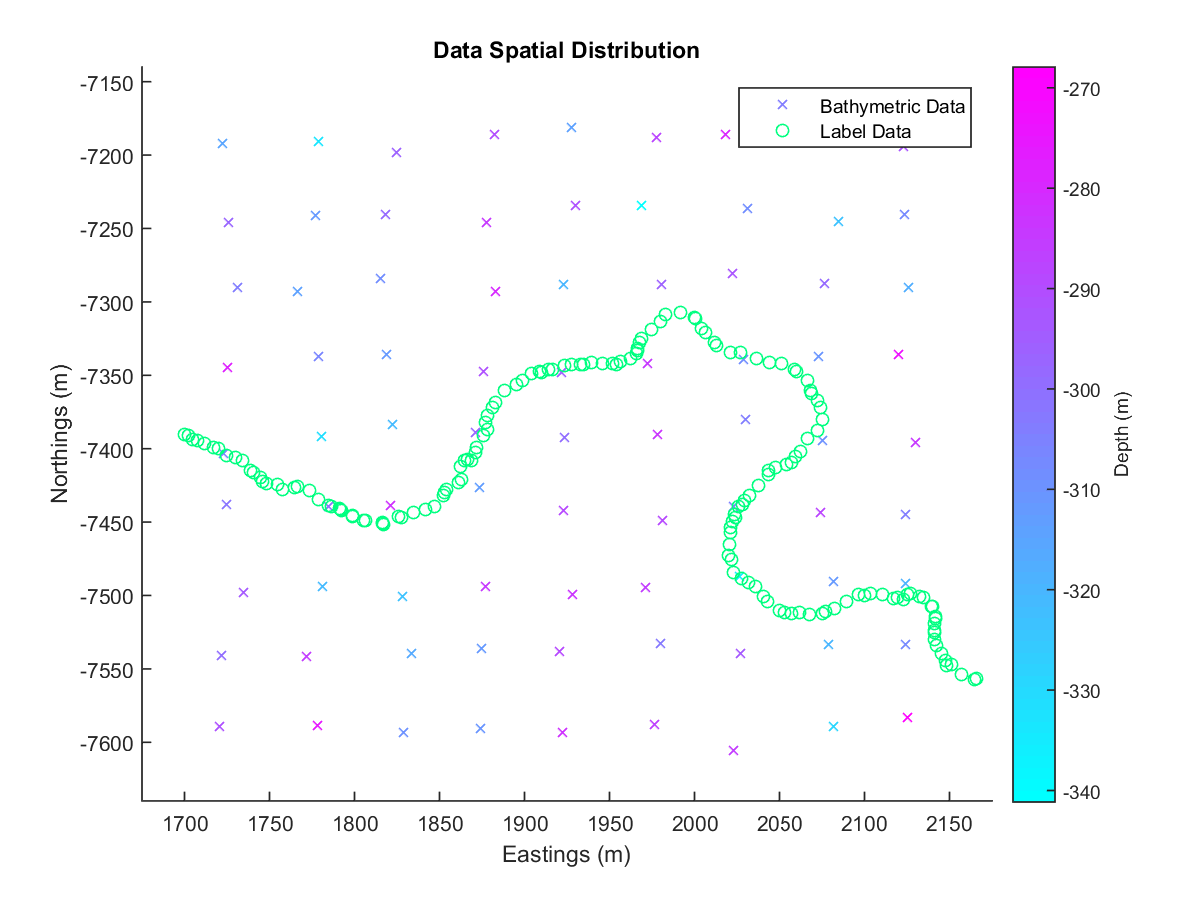
\includegraphics[width=0.9\textwidth]{Figures/illustrationBathymetricAgainstLabels.png}
				\caption{Illustration of Bathymetric and Label Data Density}
				\label{Background:OceanEnvironmentModeling:Figure:illustrationBathymetricAgainstLabels}
			\end{figure}
			
			While bathymetric data are usually collected rather uniformly, the label data are collected from past AUV missions whose trajectory are continuous curves across the ocean floor \citep{Squidle}. Due to slower AUV velocity as compared to surface ships which often employ SONAR or LIDAR techniques for bathymetry mapping, the label data are also spatially denser and concentrated on the mission trajectory, while being almost non-existent elsewhere.
			
			Therefore, in order to predict label data, the training data would need to be matched accurately. There are two straight forward choices at hand. The first is to estimate the bathymetric features at places where label data exists. However, at places near past mission paths, bathymetric data appears much more sparsely than label data, so that the feature extraction or regression prediction will yield very similar features across manly label data points. This reduces prediction power through a slow varying and limited feature group.
			
			Instead, the second choice is to estimate the label data at places where bathymetric data exists. In this setting, regions closer to past mission paths have higher volumes of label data, increasing the amount of training points. Regions further away would naturally generate more prediction uncertainty in the prediction stage.
			
			Hence, second method is chosen to be employed for data matching, in order to form our training set. Naturally, to predict environment labels from bathymetric features, we again need the Gaussian process classification model.
			
			\FloatBarrier
	
		\subsection{Feature Extraction}
		\label{Background:OceanEnvironmentModeling:FeatureExtraction}
		
			The feature extraction process assumes that the bathymetric depth data is available in grid form. That is, one can represent the available depth data $H = \{h_{k}\}_{k \in {1, 2, ..., N}}$ as $H = \{h_{ij}\}_{i \in {1, 2, ..., n_{i}}, \;\; j \in {1, 2, ..., n_{j}}}$ where varying $i$ and $j$ corresponds to varying data points in axis 1 and 2 respectively. Axis 1 and 2 is required to form an orthonormal frame. While axis 1 and 2 is usually aligned with the eastings-northings frame, it is generally not required for the feature extraction process.
			
			Without loss of generality, let $x$ and $y$ denote quantities corresponding to the orthogonal axes. We have that at $(x_{i}, y_{j})$ $(i \in {1, 2, ..., n_{i}}, \;\; j \in {1, 2, ..., n_{j}})$ the depth is measured as $h_{ij}$. The partial derivatives of various degrees of accuracy and scale can then be estimated through central differencing, as shown in \cref{Background:OceanEnvironmentModeling:Figure:centraldifferencecofficients} \citep{CentralDifferenceTable}. The author has chosen $N = 3$ neighbors for short scale slope and $N = 9$ neighbors for large scale slope.
			
			\begin{figure}[!htbp]
				\centering
					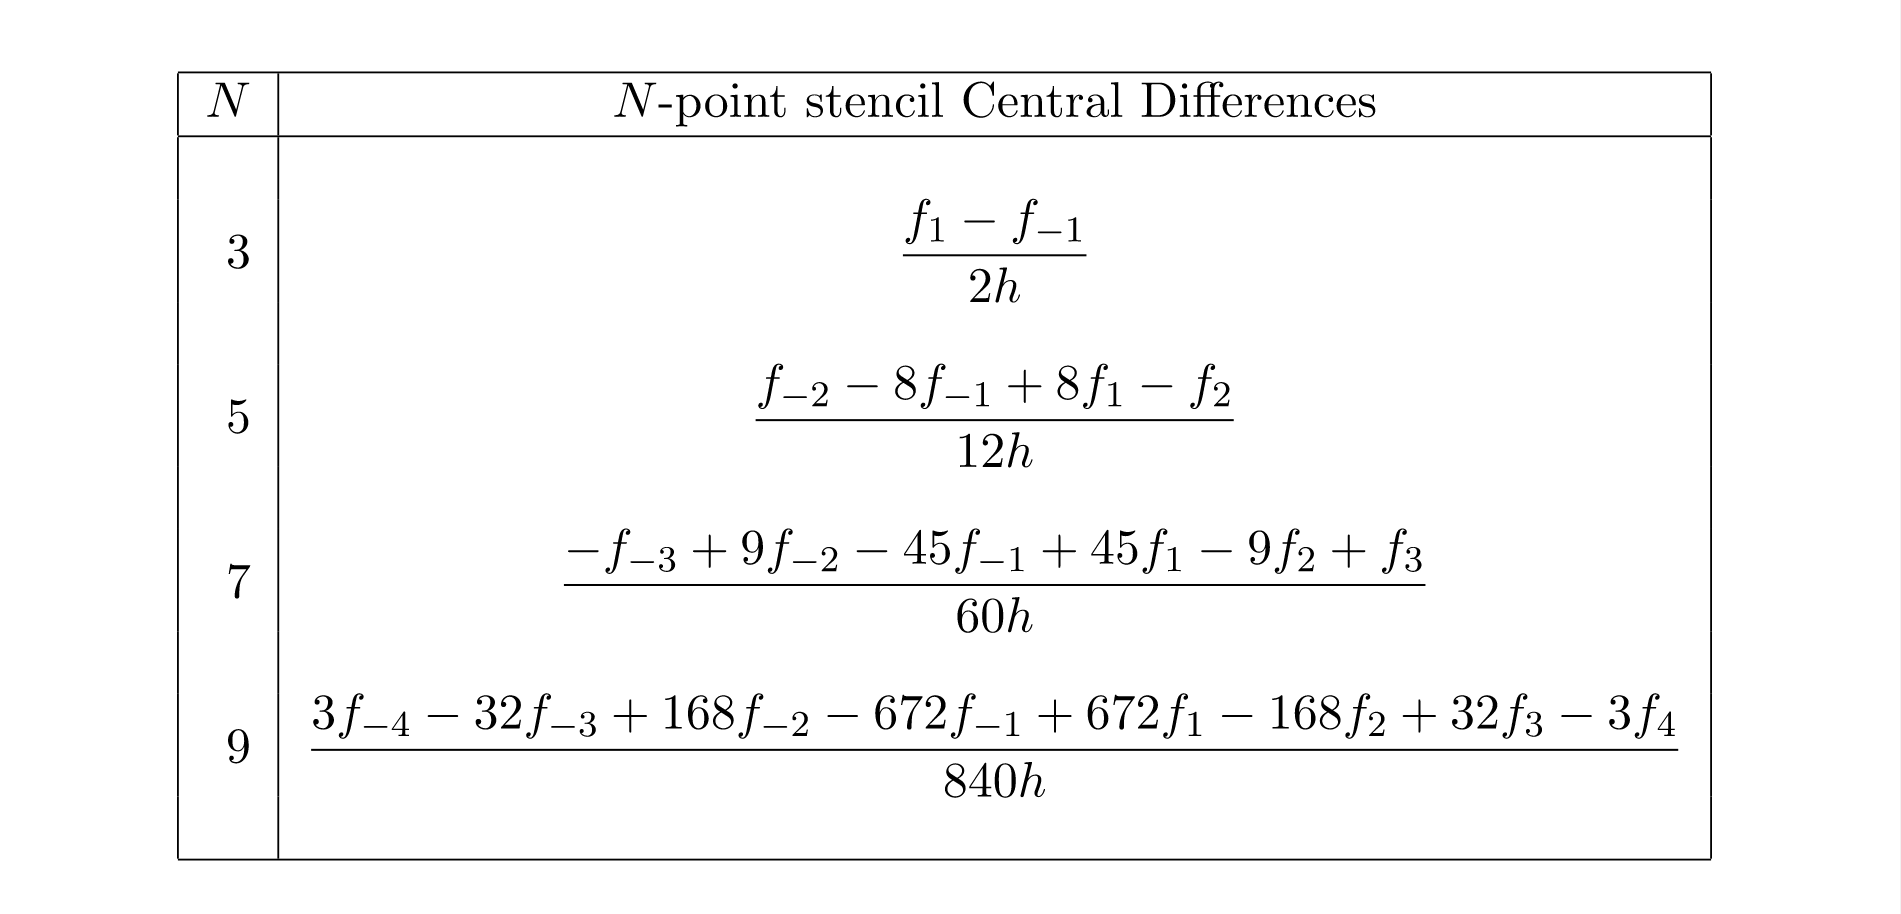
\includegraphics[width=0.9\textwidth]{Figures/centraldifferencecofficients.png}
				\caption{Finite Difference Methods: Central Difference Coefficients \\
				The subscripts $i$ represents  }
				\label{Background:OceanEnvironmentModeling:Figure:centraldifferencecofficients}
			\end{figure}			

			Central differencing is chosen as it is more numerically accurate. The disadvantages of instability and slightly higher time complexity from dynamic cases are not present in the static feature extraction process. Nevertheless, forward differencing is to be used at the boundaries of the dataset where neighboring data is missing on one side.
						
			With two axis, the result is a 2 element gradient vector. It is possible to treat the 2 elements as separate features. However, this would make the modeling problem frame dependent unnecessarily. Therefore, the magnitude of this gradient vector is taken as the slope feature. 
			
			Rugosity is a measure of local height variations in the terrain. By definition, its form is computed as $r = A_{r}/A_{g}$, the real surface area divided by the geometric surface area.
			
			Under cases without perfect grid formation, such as that shown in \cref{Background:OceanEnvironmentModeling:Figure:illustrationBathymetricAgainstLabels}, this feature extraction process becomes only an approximation. As the data set deviates from the form assumed above, it can then become necessary to estimate the features using Gaussian process regression - specifically, the multi-task Gaussian process regression. 
			
		 	On the other hand, under fine-scale bathymetric reconstructions, more sophisticated methods for deriving multi-scale measures of rugosity and slope exist. For example, under bathymetry measurements that are geo-referenced through stereo imagery, rugosity can be calculated through a Delaunay triangulated surface mesh and projecting areas onto the plane of best fit using Principal Component Analysis (PCA) \citep{StefanWilliams:Rugosity}.
							
			\FloatBarrier
				
	\section{GP Classification with Laplace Approximation}
	
		\subsection{Theory}
		
		\subsection{Implementation}
		
		\subsection{Results}
		
	\section{GP Classification with Probabilistic Least Squares Approximation}

		\subsection{Theory}
		
		\subsection{Implementation}
			
		\subsection{Results}
				
	\section{Drawing from Gaussian Process Classifiers}
				
		\subsection{Theory}
		
		\subsection{Implementation}
			
		\subsection{Results}

	\section{Laplace Approximation and Probabilistic Least Squares}
	
		Compare probability outputs, classification outputs, entropy outputs, etc

	\section{The One Versus All Framework}
	
	\section{The All Versus All Framework}
	
	\section{Properties and Performance of OVA and AVA Classifiers}
	
	\section{Probability Fusion Methods}
	
		\subsection{Normalisation Method}
			
		\subsection{Mode Keeping}
			
		\subsection{Exclusion}
			
	\section{Mapping Scott Reef Benthic Habitats}
	
		\subsection{Problems and Solutions to Big Data Analysis}
		
		\subsection{Feature Extraction}
		
		\subsection{Case with 4 Labels}
		
			(With different amounts of sampled points)
			
		\subsection{Case with 17 Labels}
		